代码见附件.

设各长度的钢管数量构成$\bm{x}\in\mathbb{R}^3$, 使得
\begin{equation*}
    \begin{pmatrix}
        2.9 & 2.1 & 1.5
    \end{pmatrix}
    \bm{x}\leq7.4,\quad x_1,x_2,x_3\text{为正整数}.
\end{equation*}
遍历所有可能的情况, 得到如\cref{table:15-1}中所示的21种可能的方案, 表中的前三列构成矩阵$\bm{A}\in\mathrm{R}^{3\times21}$, 第五列构成向量$\bm{c}\in\mathrm{R}^{21}$.
\begin{table}[ht]
    \centering
    \caption{制作100套钢架问题中可能的方案}
    \label{table:15-1}
    \resizebox{\textwidth}{!}{
        \begin{tabular}{cccccc}
            \toprule
            2.9m钢管数量 & 2.1m钢管数量 & 1.5m钢管数量 & 消耗长度(m) & 剩余长度(m) & 方案执行次数 \\
            \midrule
            0 & 0 & 1 & 5.9 & 1.5 & 0 \\
            0 & 0 & 2 & 4.4 & 3.0 & 0 \\
            0 & 0 & 3 & 2.9 & 4.5 & 0 \\
            0 & 0 & 4 & 1.4 & 6.0 & 0 \\
            0 & 1 & 0 & 5.3 & 2.1 & 0 \\
            0 & 1 & 1 & 3.8 & 3.6 & 0 \\
            0 & 1 & 2 & 2.3 & 5.1 & 0 \\
            0 & 1 & 3 & 0.8 & 6.6 & 0 \\
            0 & 2 & 0 & 3.2 & 4.2 & 0 \\
            0 & 2 & 1 & 1.7 & 5.7 & 0 \\
            0 & 2 & 2 & 0.2 & 7.2 & 0 \\
            0 & 3 & 0 & 1.1 & 6.3 & 0 \\
            1 & 0 & 0 & 4.5 & 2.9 & 0 \\
            1 & 0 & 1 & 3.0 & 4.4 & 0 \\
            1 & 0 & 2 & 1.5 & 5.9 & 0 \\
            1 & 0 & 3 & 0.0 & 7.4 & 30 \\
            1 & 1 & 0 & 2.4 & 5.0 & 0 \\
            1 & 1 & 1 & 0.9 & 6.5 & 0 \\
            1 & 2 & 0 & 0.3 & 7.1 & 50 \\
            2 & 0 & 0 & 1.6 & 5.8 & 0 \\
            2 & 0 & 1 & 0.1 & 7.3 & 10 \\
            \bottomrule
        \end{tabular}
    }
\end{table}

设每种方案执行次数构成$\bm{y}\in\mathrm{R}^{21}$, 为了使材料最省, 则只需让$\bm{c}^\mathrm{T}\bm{y}$最小, 因此得到优化问题
\optmodule{\min}{\bm{c}^\mathrm{T}\bm{y}}{
    &\bm{Ay}=100\bm{J}, \\
    &y_1,y_2,\cdots,y_{21}\text{为正整数},
    \label{equation:15-1}
}
其中$\bm{J}\in\mathrm{R}^{21}$为全1向量.

使用Julia编写程序并求解\cref{equation:15-1}, 得到\cref{table:15-1}中的第六列, 该列表示\cref{equation:15-1}的最优解$\bm{y}^*$.

因此, 最优值为
\begin{equation*}
    \bm{c}^\mathrm{T}\bm{y}^*=16,
\end{equation*}
即浪费了16m的钢管, 共消耗了$\bm{J}^\mathrm{T}\bm{y}^*=90$根钢管.

\begin{figure}[ht]
    \centering
    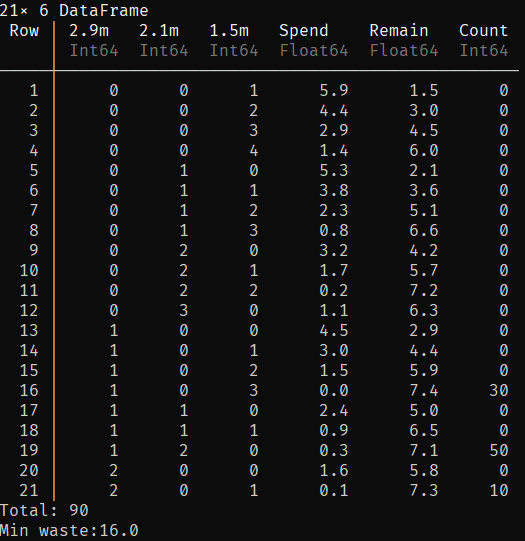
\includegraphics[scale=0.6]{figures/15-1.png}
    \caption{}
    \label{figure:15-1}
\end{figure}

程序运行输出如\cref{figure:15-1}所示.
